%!TEX TS-program = xelatex
\documentclass[12pt,a4paper, oneside]{extreport}

%%%%%%%%%% Програмный код %%%%%%%%%%
% \usepackage{minted}
% Включает подсветку команд в программах!
% Нужно, чтобы на компе стоял питон, надо поставить пакет Pygments, в котором он сделан, через pip.

% Для Windows: Жмём win+r, вводим cmd, жмём enter. Открывается консоль.
% Прописываем pip install Pygments
% Заходим в настройки texmaker и там прописываем в PdfLatex или XelaTeX:
% pdflatex -shell-escape -synctex=1 -interaction=nonstopmode %.tex

% Для Linux: Открываем консоль. Убеждаемся, что у вас установлен pip командой pip --version
% Если он не установлен, ставим его: sudo apt-get install python-pip
% Ставим пакет sudo pip install Pygments

% Для Mac: Всё то же самое, что на Linux, но через brew.

% После всего этого вы должны почувствовать себя тру-программистами!
% Документация по пакету хорошая. Сам читал, погуглите!

%%%%%%%%%% Математика %%%%%%%%%%
\usepackage{amsmath,amsfonts,amssymb,amsthm,mathtools}
% Показывать номера только у тех формул, на которые есть \eqref{} в тексте.
%\mathtoolsset{showonlyrefs=true}
%\usepackage{leqno} % Нумерация формул слева


%%%%%%%%%% Шрифты %%%%%%%%
\usepackage{fontspec}         % пакет для подгрузки шрифтов

\defaultfontfeatures{Mapping=tex-text}
\setmainfont{Times New Roman}       % задаёт основной шрифт документа

% Зачем на нужна команда \newfontfamily:
% http://tex.stackexchange.com/questions/91507/
\newfontfamily{\cyrillicfonttt}{Times New Roman}
\newfontfamily{\cyrillicfont}{Times New Roman}
\newfontfamily{\cyrillicfontsf}{Times New Roman}

\usepackage{unicode-math}     % пакет для установки математического шрифта
\setmathfont[math-style=ISO]{Asana Math}      % шрифт для математики

% Конкретный символ из конкретного шрифта
% \setmathfont[range=\int]{Neo Euler}

\usepackage{polyglossia}      % Пакет для выбора языка
% Основной язык документа. В опциях активируются всякие приколы для русского языка (вроде кучи разновидностей тире) из пакета babel
\setdefaultlanguage[babelshorthands=true]{russian}
\setotherlanguage{english}    % Второстепенный язык документа


%%%%%%%%%% Работа с картинками %%%%%%%%%
\usepackage{graphicx}                  % Для вставки рисунков
\usepackage{graphics}
\graphicspath{{images/}{pictures/}}    % можно указать папки с картинками
\usepackage{wrapfig}                   % Обтекание рисунков и таблиц текстом


%%%%%%%%%% Работа с таблицами %%%%%%%%%%
\usepackage{tabularx}            % новые типы колонок
\usepackage{tabulary}            % и ещё новые типы колонок
\usepackage{array,delarray}      % Дополнительная работа с таблицами
\usepackage{longtable}           % Длинные таблицы
\usepackage{multirow}            % Слияние строк в таблице
\usepackage{float}               % возможность позиционировать объекты в нужном месте

\usepackage{booktabs}            % таблицы как в книгах
% Заповеди из документации к booktabs:
% 1. Будь проще! Глазам должно быть комфортно
% 2. Не используйте вертикальные линни
% 3. Не используйте двойные линии. Как правило, достаточно трёх горизонтальных линий
% 4. Единицы измерения - в шапку таблицы
% 5. Не сокращайте .1 вместо 0.1
% 6. Повторяющееся значение повторяйте, а не говорите "то же"
% 7. Есть сомнения? Выравнивай по левому краю!

%  вычисляемые колонки по tabularx
\newcolumntype{C}{>{\centering\arraybackslash}X}
\newcolumntype{L}{>{\raggedright\arraybackslash}X}
\newcolumntype{Y}{>{\arraybackslash}X}
\newcolumntype{Z}{>{\centering\arraybackslash}X}


%%%%%%%%%% Графика и рисование %%%%%%%%%%
\usepackage{tikz, pgfplots}      % язык для рисования графики из latex'a

%%%%%%%%%% Гиперссылки %%%%%%%%%%
\usepackage{xcolor}              % разные цвета

\usepackage{hyperref}
\hypersetup{
    unicode=true,           % позволяет использовать юникодные символы
    colorlinks=true,       	% true - цветные ссылки, false - ссылки в рамках
    urlcolor =blue,         % цвет ссылки на url
    linkcolor=black,        % внутренние ссылки
    citecolor=black,        % на библиографию
	breaklinks              % если ссылка не умещается в одну строку, разбивать ли ее на две части?
}


%%%%%%%%%% Другие приятные пакеты %%%%%%%%%
\usepackage{multicol}       % несколько колонок
\usepackage{verbatim}       % для многострочных комментариев
\usepackage{cmap}           % для кодировки шрифтов в pdf

\usepackage{enumitem} % дополнительные плюшки для списков
%  например \begin{enumerate}[resume] позволяет продолжить нумерацию в новом списке

\usepackage{todonotes} % для вставки в документ заметок о том, что  осталось сделать
% \todo{Здесь надо коэффициенты исправить}
% \missingfigure{Здесь будет Последний день Помпеи}
% \listoftodos --- печатает все поставленные \todo'шки



%%%%%%%%%%%%%% ГОСТОВСКИЕ ПРИБАМБАСЫ %%%%%%%%%%%%%%%

%%% размер листа бумаги
\usepackage[paper=a4paper,top=15mm, bottom=15mm,left=35mm,right=10mm,includehead,includefoot]{geometry}

\usepackage{setspace}
\setstretch{1.33}     % Межстрочный интервал
\setlength{\parindent}{1.5em} % Красная строка.


\flushbottom       % Эта команда заставляет LaTeX чуть растягивать строки, чтобы получить идеально прямоугольную страницу
\righthyphenmin=2  % Разрешение переноса двух и более символов
\widowpenalty=10000  % Наказание за вдовствующую строку (одна строка абзаца на этой странице, остальное --- на следующей)
\clubpenalty=10000  % Наказание за сиротствующую строку (омерзительно висящая одинокая строка в начале страницы)
\tolerance=1000     % Ещё какое-то наказание.


% Нумерация страниц сверху по центру
\usepackage{fancyhdr}
\pagestyle{fancy}
\fancyhead{ } % clear all fields
\fancyfoot{ } % clear all fields
\fancyhead[C]{\thepage}
% Чтобы не прорисовывалась черта! 
\renewcommand{\headrulewidth}{0pt}


% Нумерация страниц с надписью "Глава"
\usepackage{etoolbox}
\patchcmd{\chapter}{\thispagestyle{plain}}{\thispagestyle{fancy}}{}{}


%%% Заголовки
\usepackage[indentfirst]{titlesec}{\raggedleft} 
% Заголовки по левому краю    
% опция identfirst устанавливает отступ в первом абзаце 

% В Linux этот пакет сделан косячно. Исправляет это следующий непонятный кусок кода. 
\makeatletter
\patchcmd{\ttlh@hang}{\parindent\z@}{\parindent\z@\leavevmode}{}{}
\patchcmd{\ttlh@hang}{\noindent}{}{}{}
\makeatother


% Редактирования Глав и названий
\titleformat{\chapter}
      {\normalfont\large\bfseries}
      {\thechapter }{0.5 em}{}

% Редактирование ненумеруемых глав chapter* (Введение и тп) 
\titleformat{name=\chapter,numberless}
{\centering\normalfont\bfseries\large}{}{0.25em}{\normalfont}
 
% Убирает чеканутые отступы вверху страницы
\titlespacing{\chapter}{0pt}{-20pt}{15 pt} 
 
% Более низкие уровни 
\titleformat{\section}{\bfseries}{\thesection}{0.5 em}{}
\titleformat{\subsection}{\bfseries}{\thesubsection}{0.5 em}{}


% Содержание. Команды ниже изменяют отступы и рисуют точечки!
\usepackage{titletoc}

\titlecontents{chapter}
             [1em] % 
             {\normalsize}
             {\contentslabel{1 em}}
             {\hspace{-1 em}}
             {\normalsize\titlerule*[10pt]{.}\contentspage}

\titlecontents{section}
              [3 em] % 
              {\normalsize}
              {\contentslabel{1.75 em}}
              {\hspace{-1.75 em}}
              {\normalsize\titlerule*[10pt]{.}\contentspage}

\titlecontents{subsection}
              [6 em] % 
              {\normalsize}
              {\contentslabel{3 em}}
              {\hspace{-3 em}}
              {\normalsize\titlerule*[10pt]{.}\contentspage}


% Правильные подписи под таблицей и рисунком
% Документация к пакету на русском языке! 
\usepackage[tableposition=top, singlelinecheck=false]{caption}
\usepackage{subcaption}

   \DeclareCaptionStyle{base}%
		[justification=centering,indention=0pt]{}
		
   \DeclareCaptionLabelFormat{gostfigure}{Рисунок #2}
   \DeclareCaptionLabelFormat{gosttable}{Таблица #2}
   
   \DeclareCaptionLabelSeparator{gost}{~---~}
   \captionsetup{labelsep=gost}

   \DeclareCaptionStyle{fig01}%
           [margin=5mm,justification=centering]%
           {margin={3em,3em}}
   \captionsetup*[figure]{style=fig01,labelsep=gost,labelformat=gostfigure,format=hang}

   \DeclareCaptionStyle{tab01}%
           [margin=5mm,justification=centering]%
           {margin={3em,3em}}
   \captionsetup*[table]{style=tab01,labelsep=gost,labelformat=gosttable,format=hang}



% межстрочный отступ в таблице
 \renewcommand{\arraystretch}{1.2}



% многостраничные таблицы под РОССИЙСКИЙ СТАНДАРТ
% ВНИМАНИЕ! Обязательно за CAPTION !
\usepackage{fr-longtable}

\makeatletter
 \LTcapwidth=\textwidth
\def\LT@makecaption#1#2#3{%
 \LT@mcol\LT@cols c{\hbox to\z@{\hss\parbox[t]\LTcapwidth{%
\sbox\@tempboxa{ #1{#2: } #3}%
 \ifdim\wd\@tempboxa>\hsize
	\hbox to\hsize{\hfil #1#2\mbox{ }}
     	\hbox to\hsize{\hfil \parbox[c]{0.9\textwidth}{\centering #3}\hfil }%%
 \else
     \hbox to\hsize{\hfil #1#2\mbox{ }}
     \hbox to\hsize{\hfil #3\hfil}%
 \fi
 \endgraf\vskip 0.5\baselineskip}%
 \hss}}}
\makeatother


%%% ГОСТОВСКИЕ СПИСКИ
% сообщаем окружению о том, что существует такая штук как нумерация русскими буквами.
\makeatletter
\AddEnumerateCounter{\asbuk}{\russian@alph}{щ}
\makeatother


% Первый тип списков. Большая буква. 
\newlist{Enumerate}{enumerate}{1}
\setlist[Enumerate,1]{labelsep=0.5em,leftmargin=1.25em,labelwidth=1.25em,
parsep=0em,itemsep=0em,topsep=0.75ex, before={\parskip=-1em},label=\arabic{Enumeratei}.}


% Второй тип списков. Маленькая буква.
\setlist[enumerate]{label=\arabic{enumi}),parsep=0em,itemsep=0em,topsep=0.75ex, before={\parskip=-1em}}


% Третий тип списков. Два уровня. 
\newlist{twoenumerate}{enumerate}{2}
\setlist[twoenumerate,1]{itemsep=0mm,parsep=0em,topsep=0.75ex,, before={\parskip=-1em},label=\asbuk{twoenumeratei})}
\setlist[twoenumerate,2]{leftmargin=1.3em,itemsep=0mm,parsep=0em,topsep=0ex, before={\parskip=-1em},label=\arabic{twoenumerateii})}


% Четвёртый тип списков. Список с тире.
\setlist[itemize]{label=--,parsep=0em,itemsep=0em,topsep=0.75ex, before={\parskip=-1em},after={\parskip=-1em}}


%%% WARNING WARNING WARNIN!
%%% Если в списке предложения, то должна по госту стоять точка после цифры => команда Enumerate! Если идет перечень маленьких фактов, не обособляемых предложений то после цифры идет скобка ")" => команда enumerate! Если перечень при этом ещё и двууровневый, то twoenumerate.




%%%%%%%%%% Список литературы %%%%%%%%%%

\usepackage[% 
backend=biber, %подключение пакета biber (тоже нужен)
bibstyle=gost-numeric, %подключение одного из четырех главных стилей biblatex-gost 
sorting=ntvy, %тип сортировки в библиографии
]{biblatex}

% Справка по 4 главным стилям для ленивых: 
% gost-inline  ссылки внутри теста в круглых скобках
% gost-footnote подстрочные ссылки
% gost-numeric затекстовые ссылки
% gost-authoryear тоже затекстовые ссылки, но немного другие 

% Подробнее смотри страницу 4 документации. Она на русском. 

% Ещё немного настроек
\DeclareFieldFormat{postnote}{#1} %убирает с. и p.
\renewcommand*{\mkgostheading}[1]{#1} % только лишь убираем курсив с авторов


\addbibresource{sc_bib.bib} % сюда нужно вписать свой bib-файлик.

% Этот кусок кода выносит русские источники на первое место. Костыль описали авторы пакета в руководстве к нему. Подробнее смотри: 
% https://github.com/odomanov/biblatex-gost/wiki/Как-сделать%2C-чтобы-русскоязычные-источники-предшествовали-остальным
\DeclareSourcemap{
  \maps[datatype=bibtex]{
    \map{
      \step[fieldsource=langid, match=russian, final]
      \step[fieldset=presort, fieldvalue={a}]
    }
    \map{
      \step[fieldsource=langid, notmatch=russian, final]
      \step[fieldset=presort, fieldvalue={z}]
    }
  }
}


%%%%%%%%% Свои команды %%%%%%%%%%%







\begin{document}

\thispagestyle{empty} % Чтобы избежать нумерации титульника

\begin{center}
\small \bfseries Федеральное государственное бюджетное образовательное учреждение высшего образования

<<РОССИЙСКАЯ АКАДЕМИЯ НАРОДНОГО ХОЗЯЙСТВА и\\ ГОСУДАРСТВЕННОЙ СЛУЖБЫ \\
при Президенте Российской Федерации>>

\vspace{2ex}

\bfseries
ЭКОНОМИЧЕСКИЙ ФАКУЛЬТЕТ

НАПРАВЛЕНИЕ 38.03.01 ЭКОНОМИКА
\end{center}

\vfill


\noindent\small Группа ЭФ-13-02
\hfill
\parbox[t]{20em}{\centering\small
Кафедра <<Макроэкономики>>

\mbox{ }

\textbf{Допустить к защите}

заведующий кафедрой <<Макроэкономики>>

\mbox{ }

\rule{8em}{0.5pt} Н.Л. Шагас

\mbox{ }

<<\rule{2em}{0.5pt}>> \rule{5em}{0.5pt} 201\rule{1em}{0.5pt} г. }

\mbox{ }

\mbox{ }

\begin{center}\bfseries
ВЫПУСКНАЯ КВАЛИФИКАЦИОННАЯ РАБОТА

\mbox{ }

\large
ТЕМА ВЫПУСКНОЙ КВАЛИФИКАЦИОННОЙ РАБОТЫ \\
ПРОДОЛЖЕНИЕ ТЕМЫ ВЫПУСКНОЙ КВАЛИФИКАЦИОННОЙ РАБОТЫ
\end{center}

\vfill

\noindent\normalsize
студент-бакалавр

\noindent
Иванов Иван Иванович
\hfill /\rule{6em}{0.5pt}/\rule{6em}{0.5pt}/

\hfill\makebox[13em]{\hfill\footnotesize (подпись) \hfill\hfill (дата) \hfill}

\noindent
научный руководитель выпускной \\
квалификационной работы

\noindent
к.э.н., доцент Сидоров Сидор Сидорович
\hfill /\rule{6em}{0.5pt}/\rule{6em}{0.5pt}/

\hfill\makebox[13em]{\hfill\footnotesize (подпись) \hfill\hfill (дата) \hfill}

%\noindent
%консультант
%
%\noindent
%д.э.н., профессор Петров Петр Петрович
%\hfill /\rule{6em}{0.5pt}/\rule{6em}{0.5pt}/
%
%\hfill\makebox[13em]{\hfill\footnotesize (подпись) \hfill\hfill (дата) \hfill}

\vfill

\begin{center}
\normalsize \bfseries МОСКВА \\ 2017 г.
\end{center}




%%%%%%%%%%%%%%%%%%% ОГЛАВЛЕНИЕ %%%%%%%%%%%%%%%%%%%%%%%%%%%%%%%%%%%%%%

\tableofcontents  % Команда, которая создаёт оглавление



%%%%%%%%%%%%%%%%%%%% ВВЕДЕНИЕ %%%%%%%%%%%%%%%%%%%%%%%%%%%%%%%%%%%%
\chapter*{Введение}
\addcontentsline{toc}{chapter}{Введение}


Магистерская диссертация является выпускной квалификационной работой, подготовленной для публичной защиты и показывает уровень профессиональной подготовки студента, умение самостоятельно вести научный поиск и решать практические задачи в сфере профессиональной деятельности. Для программы <<Экономика и финансы>> видом профессиональной деятельности является научно-исследовательская и аналитическая. Магистерская диссертация является формой итогового контроля за обучением студентов.


\chapter{Название главы}

\section{Название пункта}

Магистерская диссертация является выпускной квалификационной работой, подготовленной для публичной защиты и показывает уровень профессиональной подготовки студента, умение самостоятельно вести научный поиск и решать практические задачи в сфере профессиональной деятельности. Для программы <<Экономика и финансы>> видом профессиональной деятельности является научно-исследовательская и аналитическая. Магистерская диссертация является формой итогового контроля за обучением студентов.


 
\subsection{Списки}

При оформлении \textbf{нумерованных списков} в магистерской диссертации следует ограничиться тремя видами списков: нумерованным списком содержащим в одном пункте несколько предложений, нумерованным списком содержащим в одном пункте одно предложение, двухуровневым нумерованным списком. Использование других  нумерованных списков не рекомендуется.

Приведем нумерованный список, содержащий в одном пункте несколько предложений:
\begin{Enumerate}
\item 	Каждый пункт нумерованного списка, содержащего в одном пункте несколько предложений должен начинаться с большой буквы и заканчиваться точкой.
\item 	Номер пункта данного списка выравнивается по левому краю без абзацного отступа. После номера ставится точка и делается отступ для написания текста. 
\item Текст списка выравнивается по ширине. В тексте используются переносы. Левая граница второй и последующих строк внутри текста пункта выравниваются по первой букве текста первой строки.
\item Все первые буквы текста первых строк пунктов списка должны быть выровнены между собой.
\end{Enumerate}


Приведем пример нумерованного списка, содержащего в одном пункте одно предложение:
	\begin{enumerate}
		\item тест списка начинается с маленькой буквы и заканчивается точкой с запятой;
		\item номер пункта списка выравнивается по левому краю с абзацным отступом;
		\item после номера ставится точка и делается отступ для написания текста;
		\item текст списка выравнивается по ширине; 
		\item в тексте используются переносы; 
		\item левая граница второй и последующих строк внутри текста пункта выравниваются по первой букве текста первой строки;
		\item все первые буквы текста первых строк пунктов списка должны быть выровнены между собой;
		\item последнее предложение оканчивается точкой.		
	\end{enumerate} 

Двухуровневый нумерованный список, используется при необходимости перечислений внутри списка. В соответствии с ГОСТ 2.105 и ГОСТ 7.32 нумеруется прописными буквами русского алфавита за исключением букв <<ё, з, й, о, ч, ъ, ы, ь>>. Приведем пример такого списка:
	\begin{twoenumerate}
		\item тест списка начинается с маленькой буквы и заканчивается точкой с запятой;
		\item номер пункта списка выравнивается по левому краю с абзацным отступом;
		\item после номера ставится точка и делается отступ для написания текста;
		\item номер второго уровня выравнивается по тексту первого уровня;
			\begin{twoenumerate}
				\item текст списка выравнивается по ширине; 
				\item в тексте используются переносы; 
				\item левая граница второй и последующих строк внутри текста пункта выравниваются по первой букве текста первой строки;
			\end{twoenumerate}
		\item все первые буквы текста первых строк пунктов списка должны быть выровнены между собой;
		\item последнее предложение оканчивается точкой.		
	\end{twoenumerate}

Ненумерованные списки используются для перечислений. Обычно в таком списке один пункт, одно предложение. Приведем пример такого списка:
\begin{itemize}
	\item в качестве маркера списка используется тире;
	\item применение других типов маркеров недопустимо; 
	\item остальное оформление списка аналогично нумерованному списку содержащему в одном пункте одно предложение.
\end{itemize}


\subsection{Библиографические ссылки}


 Библиографическая ссылка является частью справочного аппарата документа и служит источником библиографической информации о документах --- объектах ссылки. Библиографическая ссылка содержит библиографические сведения о цитируемом, рассматриваемом или упоминаемом в тексте документа другом документе (его составной части или группе документов), необходимые и достаточные 

Библиографические ссылки в тексте магистерской диссертации оформляют в соответствии с требованиями ГОСТ Р 7.0.5.

По месту расположения в документе различают библиографические ссылки  следующего типа:  
\begin{itemize}
\item внутритекстовые, помещенные в тексте документа; 
\item подстрочные, вынесенные из текста вниз полосы документа (в сноску);
\item затекстовые, вынесенные за текст документа или его части (в выноску).	
\end{itemize}

В диссертации допускается использование \textbf{только одного типа} библиографических ссылок. Рекомендуется в диссертации  использовать  \textbf{внутритекстовые или подстрочные} ссылки на библиографические источники. 

Внутритекстовая библиографическая ссылка может содержать следующие элементы:
\begin{itemize}
\item заголовок;
\item основное заглавие документа;
\item общее обозначение материала;
\item сведения об ответственности;
\item сведения об издании;
\item выходные данные;
\item сведения об объеме документа (если ссылка на весь документ);
\item сведения о местоположении объекта ссылки в документе (если ссылка на часть документа);
\item обозначение и порядковый номер тома или выпуска (для ссылок на публикации в многочастных или сериальных документах);
\item сведения о документе, в котором опубликован объект ссылки;
\item примечания.	
\end{itemize}

Внутритекстовую библиографическую ссылку заключают в круглые скобки. Элементы 
библиографической ссылки отделяются точкой. Например:

(Аренс В. Ж. Азбука исследователя. М.: Интермет Инжиниринг, 2006)

(Потемкин В. К., Казаков Д. Н. Социальное партнерство: формирование, оценка, регулирование. СПб., 2002. 202 с.)

(Собрание сочинений. М. : Экономика, 2006.  Т. 1. С. 24–56)



Подстрочная библиографическая ссылка оформляется как примечание, вынесенное из текста документа вниз полосы.
Подстрочная библиографическая ссылка может содержать следующие элементы:
\begin{itemize}
\item заголовок;
\item основное заглавие документа;
\item общее обозначение материала;
\item сведения, относящиеся к заглавию;
\item сведения об ответственности;
\item сведения об издании;
\item выходные данные;
\item сведения об объеме документа (если ссылка на весь документ);
\item сведения о местоположении объекта ссылки в документе (если ссылка на часть документа);
\item сведения о серии;
\item обозначение и порядковый номер тома или выпуска (для ссылок на публикации в многочастных или сериальных документах);
\item сведения о документе, в котором опубликован объект ссылки; 
\item примечания;
\item Международный стандартный номер.
\end{itemize}

В подстрочной библиографической ссылке повторяют имеющиеся в тексте документа библиографические сведения об объекте ссылки. 

\textsuperscript{3}~Аренс В. Ж. Азбука исследователя. М.: Интермет Инжиниринг, 2006.

\textsuperscript{5}~Потемкин В. К., Казаков Д. Н. Социальное партнерство: формирование, оценка, регулирование. СПб., 2002. 202 с.)

\textsuperscript{6}~Собрание сочинений. М. : Экономика, 2006.  Т. 1. С. 24–56)

Сноски в тексте магистерской диссертации могут нумероваться:
\begin{itemize}
\item постранично, на каждой странице по отдельности начиная с единицы;
\item сквозным способом, каждая ссылка имеет свой порядковый номер, начиная с единицы. 
\end{itemize}

В магистерской диссертации рекомендуется использовать \textbf{сквозную} нумерацию ссылок.

О правилах оформления затекстовых ссылок можно узнать в ГОСТ Р 7.0.5.

Повторную ссылку на один и тот же документ (группу документов) или его часть, приводят в сокращенной форме при условии, что все необходимые для идентификации и поиска этого документа библиографические сведения указаны в первичной ссылке на него. Выбранный прием сокращения библиографических сведений используется единообразно для данного документа.

Например:

для внутритекстовых ссылок

\noindent \textit{Первичная}

(Герасимов Б. Н., Морозов В. В., Яковлева Н. Г. Системы управления: понятия, структура, исследование. Самара, 2002)

\noindent \textit{Повторная}

(Герасимов Б. Н., Морозов В. В., Яковлева Н. Г. Системы управления ... С. 53–54)

\noindent \textit{Первичная}

для подстрочных ссылок

\textsuperscript{8} Геоинформационное моделирование территориальных рынков банковских услуг~/ А.Г. Дружинин [и др.]. Шахты : Изд-во ЮРГУЭС, 2006.

\noindent \textit{Повторная}

\textsuperscript{12} Геоинформационное моделирование … С. 28.

Все источники указанные в библиографических ссылках должны быть указана в списке литературы. 

Заимствования, сделанные в диссертации без указания библиографической ссылки на первоисточник, являются плагиатом. \textbf{Магистерская диссертация уличенная в плагиате снимается с защиты без права повторной защиты.}

Пример ссылки на источник из текста.

По структуре доклад можно разделить на три части\footnote{Аристер Н.И., Резник С.Д. Управление диссертационным советом: Практическое пособие / под общ. Ред. Проф. Ф.И. Шахматова. --- 4-е изд., перераб. и доп. --- М.: ИНФРА–М., 2011. С. 91–92}. Каждая часть представляет собой самостоятельный смысловой блок, хотя в целом они логически взаимосвязаны и отражают содержание проведенного исследования.

\subsection{Иллюстрации}


Пример оформления иллюстрации с подрисуночной надписью в одну строку приведен на рисунке \ref{ris:02:01}  и с подрисуночной надписью в несколько строк --- на рисунке \ref{ris:02:02}.

\begin{figure}[H]
  \centering
    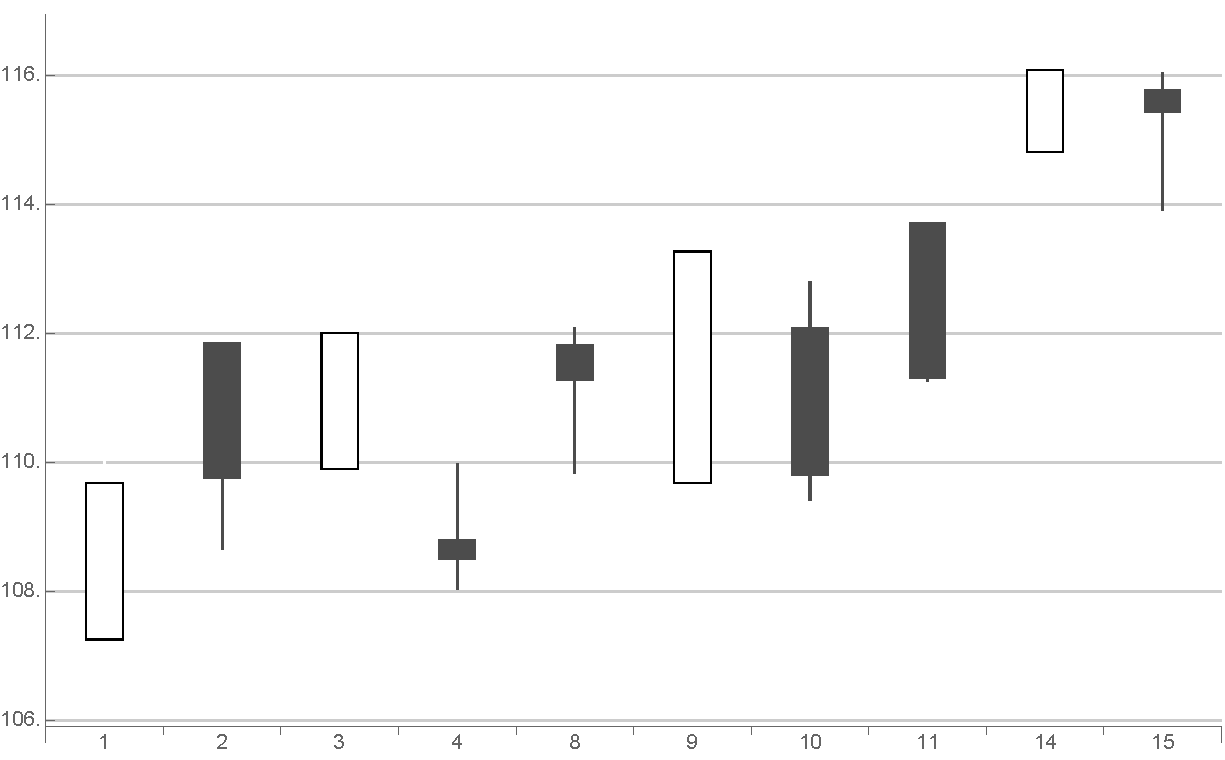
\includegraphics [width=0.5\linewidth]{Ris-01}
  \caption{Стоимость акций }\label{ris:02:01}
\end{figure}

\begin{figure}[H]
  \centering
    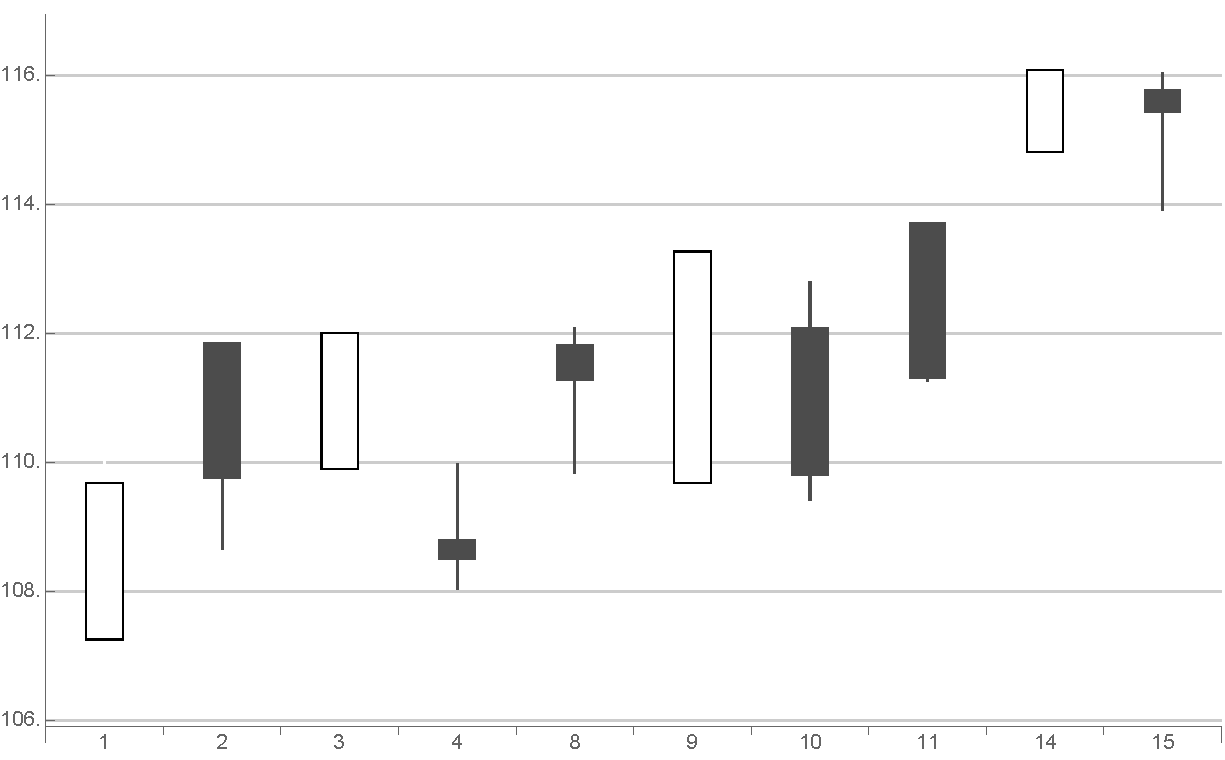
\includegraphics [width=0.5\linewidth]{Ris-01}
  \caption{Стоимость акций компании Apple на бирже NASDAQ с 1 по 15 сентября 2015 г.}\label{ris:02:02}
\end{figure}


\subsection{Таблицы}

 
Перечень таблиц указывают в списке иллюстративного материала. \footnote{Аристер Н.И., Резник С.Д. Управление диссертационным советом: Практическое пособие / под общ. Ред. Проф. Ф.И. Шахматова. --- 4-е изд., перераб. и доп. --- М.: ИНФРА–М., 2011. С. 91–92} Пример оформления приведен в таблице \ref{tab:02:01}.


\begin{table}[H]
\caption{Матрица $X$ исходных данных для решения задачи выбора вариантов данных}\label{tab:02:01}
  \centering
\begin{tabular}%{\linewidth}
{|c|c|c|c|c|c|c|c|}\hline
1	& $x_{11}$ & $x_{12}$ & ... & $x_{1j}$ & ... & $x_{1,m-1} $ & $x_{1,m}$\\\hline
2	& $x_{21}$ & $x_{22}$ & ... & $x_{2j}$ & ... & $x_{2,m-1} $ & $x_{2,m}$\\\hline
3	& $x_{31}$ & $x_{32}$ & ... & $x_{3j}$ & ... & $x_{3,m-1} $ & $x_{3,m}$\\\hline
...&...&...&...&...&...&...&...\\\hline
i	& $x_{i1}$ & $x_{i2}$ & ... & $x_{ij}$ & ... & $x_{i,m-1} $ & $x_{i,m}$\\\hline
...&...&...&...&...&...&...&...\\\hline
$n-1$	& $x_{n-1,1}$ & $x_{n-1,2}$ & ... & $x_{n-1,j}$ & ... & $x_{n-1,m-1} $ & $x_{n-1,m}$\\\hline
$n$      & $x_{n,1}$ & $x_{n,2}$ & ... & $x_{n,j}$ & ... & $x_{n,m-1} $ & $x_{n,m}$\\\hline
\end{tabular}
\end{table}


\begin{table}[H]
\caption{Матрица $X$ исходных данных}\label{tab:02:01}
  \centering
\begin{tabular}%{\linewidth}
{|c|c|c|c|c|c|c|c|}\hline
1	& $x_{11}$ & $x_{12}$ & ... & $x_{1j}$ & ... & $x_{1,m-1} $ & $x_{1,m}$\\\hline
2	& $x_{21}$ & $x_{22}$ & ... & $x_{2j}$ & ... & $x_{2,m-1} $ & $x_{2,m}$\\\hline
3	& $x_{31}$ & $x_{32}$ & ... & $x_{3j}$ & ... & $x_{3,m-1} $ & $x_{3,m}$\\\hline
...&...&...&...&...&...&...&...\\\hline
i	& $x_{i1}$ & $x_{i2}$ & ... & $x_{ij}$ & ... & $x_{i,m-1} $ & $x_{i,m}$\\\hline
...&...&...&...&...&...&...&...\\\hline
$n-1$	& $x_{n-1,1}$ & $x_{n-1,2}$ & ... & $x_{n-1,j}$ & ... & $x_{n-1,m-1} $ & $x_{n-1,m}$\\\hline
$n$      & $x_{n,1}$ & $x_{n,2}$ & ... & $x_{n,j}$ & ... & $x_{n,m-1} $ & $x_{n,m}$\\\hline
\end{tabular}
\end{table}




При переносе части таблицы на другой лист (страницу) слово «Таблица» и номер ее указывают один раз справа над первой частью таблицы, над другими частями пишут слово «Продолжение», а над последней частью таблицы <<Окончание>>. После слова «Продолжение» (<<Окончание>>) указывают номер\footnote{Аристер Н.И., Резник С.Д. Управление диссертационным советом: Практическое пособие / под общ. Ред. Проф. Ф.И. Шахматова. --- 4-е изд., перераб. и доп. --- М.: ИНФРА–М., 2011. С. 91–92} таблицы, например: «Продолжение таблицы 2.3» («Окончание таблицы 2.3»).

\begin{table}[H]
\caption{Основные технико-экономические показатели ОАО «Альфа»}\label{tab}
  \small\centering\setlength{\extrarowheight}{0.25em}
\begin{tabular}%{\linewidth}
{|p{14em}|p{5em}|p{5em}|p{10em}|}\hline
\centering Показатели &
\centering 2006 год &
\centering	2007 год	 & 
\centering\arraybackslash  Темп прироста, \% \\\hline
\centering 1  &\centering 2&\centering 3 &\centering\arraybackslash 4 \\\hline
1. Объем производства, тыс. т. &\centering	1596 &\centering	1879 &\centering\arraybackslash	+17,7 \% \\\hline
\centering ...  &\centering ... &\centering ...  &\centering\arraybackslash ... \\\hline
\end{tabular}
\end{table}

\hfill ----------------- \textit{разрыв страницы} ----------------- \hfill { }

\begin{table}[H]
  \small\centering\setlength{\extrarowheight}{0.25em}
\begin{tabular}%{\linewidth}
{|p{14em}|p{5em}|p{5em}|p{10em}|}
\multicolumn{4}{r}{\normalsize Продолжение таблицы \ref{tab}}\\\hline
\centering 1  &\centering 2&\centering 3 &\centering\arraybackslash 4 \\\hline
4. Затраты на производство, млн. руб. &\centering	100 & \centering	118&	\centering\arraybackslash +18 \% \\\hline
\centering ...  &\centering ... &\centering ...  &\centering\arraybackslash ... \\\hline
\end{tabular}
\end{table}

\hfill ----------------- \textit{разрыв страницы} ----------------- \hfill { }

\begin{table}[H]
  \small\centering\setlength{\extrarowheight}{0.25em}
\begin{tabular}%{\linewidth}
{|p{14em}|p{5em}|p{5em}|p{10em}|}
\multicolumn{4}{r}{\normalsize Окончание таблицы \ref{tab}}\\\hline
\centering 1  &\centering 2&\centering 3 &\centering\arraybackslash 4 \\\hline
10. Выручка от продаж, млн. руб. &\centering	941 & \centering	1284&	\centering\arraybackslash +36.5 \% \\\hline
\end{tabular}
\end{table}


Допускается уменьшение шрифта текста внутри таблицы до шрифта размером 10pt. Допускается подписывать колонки таблиц, располагая текст с поворотом на 90 градусов --- вертикально, снизу вверх.

Пример  кода многостраничной таблицы fr-longtable

\begin{longtable}
{|>{\centering\footnotesize}p{3em}
 |>{\centering\footnotesize}p{4em}
 |>{\centering\footnotesize}p{8em}
 |>{\centering\footnotesize}p{4.4em}
 |>{\centering\footnotesize}p{4em}
 |>{\centering\footnotesize\arraybackslash}p{4em}|
}
\caption{Таблица тарифов интернет-провайдеров в Москве}\label{ltab}\\

\hline
Номер предложения & Компания & Названиe тарифа & Цена & Скорость входящего трафика &Скорость исходящего трафика
\\\hline
\endfirsthead

\multicolumn{6}{r}{Продолжение таблицы \ref{ltab}}\\\hline
Номер предложения & Компания & Названиe тарифа & Цена & Скорость входящего трафика &Скорость исходящего трафика
\\\hline
\endhead

\multicolumn{6}{r}{Окончание таблицы \ref{ltab}}\\\hline
Номер предложения & Компания & Названиe тарифа & Цена & Скорость входящего трафика &Скорость исходящего трафика
\\\hline
\endlasthead


1&2Ком (2kom)&Скоростной& 650 руб/мес.& 30 Мб/c& 30 Мб/c\\\hline
2&&50х50& 850 руб/мес.& 50 Мб/c& 50 Мб/c\\\hline
3&&ЖАЖДА СКОРОСТИ& 950 руб/мес.& 75 Мб/c& 75 Мб/c\\\hline
4&&ПРОСТО 5& 350 руб/мес.& 5 Мб/c& 5 Мб/c\\\hline
5&&То, что надо& 390 руб/мес.& 10 Мб/c& 10 Мб/c\\\hline
6&&ЛЮБИМЫЙ& 450 руб/мес.& 15 Мб/c& 15 Мб/c\\\hline
7&&CRAZY NIGHT& 450 руб/мес.& 10 Мб/c& 10 Мб/c\\\hline
8&&Поддай скорости!& 490 руб/мес.& 20 Мб/c& 20 Мб/c\\\hline
9&&Умножай на 2& 600 руб/мес.& 25 Мб/c& 25 Мб/c\\\hline
10&&РЕЗИНОВОЕ ЛЕТО& 600 руб/мес.& 20 Мб/c& 20 Мб/c\\\hline
11&&ЭКОНОМНЫЙ& 390 руб/мес.& 5 Мб/c& 5 Мб/c\\\hline
12&&РАЦИОНАЛЬНЫЙ& 490 руб/мес.& 10 Мб/c& 10 Мб/c\\\hline
13&&ДОМАШНИЙ& 650 руб/мес.& 15 Мб/c& 15 Мб/c\\\hline
14&&ДЕЛОВОЙ& 790 руб/мес.& 20 Мб/c& 20 Мб/c\\\hline
15&&СТАНДАРТ& 1200 руб/мес.& 30 Мб/c& 30 Мб/c\\\hline
16&&ПРОФЕССИОНАЛ& 2150 руб/мес.& 50 Мб/c& 50 Мб/c\\\hline
17&Авакс-телеком (Avax Telecom)&Б-300& 300 руб/мес.& 2 Мб/c& 2 Мб/c\\\hline
18&&Б-400& 400 руб/мес.& 4 Мб/c& 4 Мб/c\\\hline
19&&Б-600& 600 руб/мес.& 8 Мб/c& 8 Мб/c\\\hline
20&&Б-700& 700 руб/мес.& 16 Мб/c& 16 Мб/c\\\hline
21&&Б-800& 800 руб/мес.& 20 Мб/c& 20 Мб/c\\\hline
22&&Б-1000& 1000 руб/мес.& 30 Мб/c& 30 Мб/c\\\hline
23&&Б-1400& 1400 руб/мес.& 40 Мб/c& 40 Мб/c\\\hline
24&АйФлэт (iFlat)&iFlat 290& 290 руб/мес.& 3 Мб/c& 3 Мб/c\\\hline
25&&iFlat 390& 390 руб/мес.& 10 Мб/c& 10 Мб/c\\\hline
26&&iFlat 490& 490 руб/мес.& 20 Мб/c& 20 Мб/c\\\hline
27&&iFlat 590& 590 руб/мес.& 40 Мб/c& 40 Мб/c\\\hline
28&&iFlat 790& 790 руб/мес.& 80 Мб/c& 80 Мб/c\\\hline
29&Академнет (AkademNet)&AkNet-290-Эконом 2& 290 руб/мес.& 2 Мб/c& 2 Мб/c\\\hline
30&&AkNet-450-Стандарт 21& 450 руб/мес.& 21 Мб/c& 21 Мб/c\\\hline
31&&AkNet-600-Премиум 30& 600 руб/мес.& 30 Мб/c& 30 Мб/c\\\hline
32&&AkNet-850-Профи 51& 850 руб/мес.& 51 Мб/c& 51 Мб/c\\\hline
33&&AkNet-950-Макси 75& 950 руб/мес.& 75 Мб/c& 75 Мб/c\\\hline
34&Акадо (Akado)&АКАДО 3& 250 руб/мес.& 3 Мб/c& 3 Мб/c\\\hline
35&&АКАДО 5& 350 руб/мес.& 5 Мб/c& 5 Мб/c\\\hline
36&&АКАДО 15& 450 руб/мес.& 15 Мб/c& 15 Мб/c\\\hline
37&&АКАДО 20& 550 руб/мес.& 20 Мб/c& 20 Мб/c\\\hline
38&&АКАДО 30& 650 руб/мес.& 30 Мб/c& 30 Мб/c\\\hline
39&&АКАДО 40& 800 руб/мес.& 40 Мб/c& 40 Мб/c\\\hline
40&&АКАДО 50& 1000 руб/мес.& 50 Мб/c& 50 Мб/c\\\hline
41&АльтерЛан (AlterLan)&Домашний& 433 руб/мес.& 15 Мб/c& 15 Мб/c\\\hline
42&&Уютный& 503 руб/мес.& 25 Мб/c& 25 Мб/c\\\hline
43&&Комфортный& 573 руб/мес.& 30 Мб/c& 30 Мб/c\\\hline
44&&Надежный& 643 руб/мес.& 60 Мб/c& 60 Мб/c\\\hline
45&Альфа Нет Телеком (Alfa Net Telecom)&XB-350& 350 руб/мес.& 1.5 Мб/c& 1 Мб/c\\\hline
46&&XB-400& 400 руб/мес.& 4.5 Мб/c& 2.5 Мб/c\\\hline
47&&XB-500& 500 руб/мес.& 8.5 Мб/c& 6 Мб/c\\\hline
48&&XB-600& 600 руб/мес.& 16 Мб/c& 10.5 Мб/c\\\hline
49&&XB-750& 750 руб/мес.& 24 Мб/c& 15 Мб/c\\\hline
50&&XB-900& 900 руб/мес.& 35 Мб/c& 20 Мб/c\\\hline
\end{longtable}

\subsection{Формулы}


Приведем примеры оформления формул.

Эластичность спроса по доходу показывает на сколько процентов изменится величина спроса при изменении дохода на 1\%:
\begin{equation}
	E=\dfrac{dQ\,/\,dI}{Q\,/\,I}\,,
\end{equation}
где $E$ -- эластичность, $Q$ -- количество, $P$ -- цена, $d$ -- изменение показателя, $I$ -- доход.

Формула Тейлора с остаточным членом в форме Лагранжа
	\begin{multline}
		f(x)=f(x_{0} )+f'(x_{0} )(x-x_{0} )+\frac{f''(x_{0} )}{2} (x-x_{0} )^{2} +...+\\
		+\frac{f^{(n)} (x_{0} )}{n!} (x-x_{0} )^{n} +\frac{f^{(n+1)} (\xi )}{(n+1)!} (x-x_{0} )^{n+1}\,.  
	\end{multline}	

Вычислим интеграл:
\begin{equation*}
\int x\sin  x\,dx=
-\int x\, d\left(\cos  x \right)=
-x \cos  x+\int \cos  x\,dx=
-x \cos  x+\sin  x+C\,.
\end{equation*}

Обратите внимание на применение различных шрифтов (прямого и наклонного) в формулах.

Более детально с правилами оформления формул можно ознакомится в ГОСТ 2.105.


%%%%%%%%%%%%%%%% Новая глава %%%%%%%%%%%%%
\chapter{Название главы}

\section{Название параграфа}

\subsection{Название пункта}

Магистерская диссертация является выпускной квалификационной работой, подготовленной для публичной защиты и показывает уровень профессиональной подготовки студента, умение самостоятельно вести научный поиск и решать практические задачи в сфере профессиональной деятельности. Для программы <<Экономика и финансы>> видом профессиональной деятельности является научно-исследовательская и аналитическая. Магистерская диссертация является формой итогового контроля за обучением студентов.

\subsection{Название пункта}

Магистерская диссертация является выпускной квалификационной работой, подготовленной для публичной защиты и показывает уровень профессиональной подготовки студента, умение самостоятельно вести научный поиск и решать практические задачи в сфере профессиональной деятельности. Для программы <<Экономика и финансы>> видом профессиональной деятельности является научно-исследовательская и аналитическая. Магистерская диссертация является формой итогового контроля за обучением студентов.

\subsection{Название пункта}

Магистерская диссертация является выпускной квалификационной работой, подготовленной для публичной защиты и показывает уровень профессиональной подготовки студента, умение самостоятельно вести научный поиск и решать практические задачи в сфере профессиональной деятельности. Для программы <<Экономика и финансы>> видом профессиональной деятельности является научно-исследовательская и аналитическая. Магистерская диссертация является формой итогового контроля за обучением студентов.



%%%%%%%%%%%%%%% Новая глава %%%%%%%%%%%%%%%%%%
\chapter{Название главы}

\section{Название параграфа}

\subsection{Название пункта}

Магистерская диссертация является выпускной квалификационной работой, подготовленной для публичной защиты и показывает уровень профессиональной подготовки студента, умение самостоятельно вести научный поиск и решать практические задачи в сфере профессиональной деятельности. Для программы <<Экономика и финансы>> видом профессиональной деятельности является научно-исследовательская и аналитическая. Магистерская диссертация является формой итогового контроля за обучением студентов.

\subsection{Название пункта}

Магистерская диссертация является выпускной квалификационной работой, подготовленной для публичной защиты и показывает уровень профессиональной подготовки студента, умение самостоятельно вести научный поиск и решать практические задачи в сфере профессиональной деятельности. Для программы <<Экономика и финансы>> видом профессиональной деятельности является научно-исследовательская и аналитическая. Магистерская диссертация является формой итогового контроля за обучением студентов.

\subsection{Название пункта}

Магистерская диссертация является выпускной квалификационной работой, подготовленной для публичной защиты и показывает уровень профессиональной подготовки студента, умение самостоятельно вести научный поиск и решать практические задачи в сфере профессиональной деятельности. Для программы <<Экономика и финансы>> видом профессиональной деятельности является научно-исследовательская и аналитическая. Магистерская диссертация является формой итогового контроля за обучением студентов.

\section{Название параграфа}

\subsection{Название пункта}

Магистерская диссертация является выпускной квалификационной работой, подготовленной для публичной защиты и показывает уровень профессиональной подготовки студента, умение самостоятельно вести научный поиск и решать практические задачи в сфере профессиональной деятельности. Для программы <<Экономика и финансы>> видом профессиональной деятельности является научно-исследовательская и аналитическая. Магистерская диссертация является формой итогового контроля за обучением студентов.

\subsection{Название пункта}

Магистерская диссертация является выпускной квалификационной работой, подготовленной для публичной защиты и показывает уровень профессиональной подготовки студента, умение самостоятельно вести научный поиск и решать практические задачи в сфере профессиональной деятельности. Для программы <<Экономика и финансы>> видом профессиональной деятельности является научно-исследовательская и аналитическая. Магистерская диссертация является формой итогового контроля за обучением студентов.

\subsection{Название пункта}

Магистерская диссертация является выпускной квалификационной работой, подготовленной для публичной защиты и показывает уровень профессиональной подготовки студента, умение самостоятельно вести научный поиск и решать практические задачи в сфере профессиональной деятельности. Для программы <<Экономика и финансы>> видом профессиональной деятельности является научно-исследовательская и аналитическая. Магистерская диссертация является формой итогового контроля за обучением студентов.



%%%%%%% Заключение %%%%%%%
\chapter*{Заключение}
% Добавляем заключение в оглавление
\addcontentsline{toc}{chapter}{Заключение}

Магистерская диссертация является выпускной квалификационной работой, подготовленной для публичной защиты и показывает уровень профессиональной подготовки студента, умение самостоятельно вести научный поиск и решать практические задачи в сфере профессиональной деятельности. Для программы <<Экономика и финансы>> видом профессиональной деятельности является научно-исследовательская и аналитическая. Магистерская диссертация является формой итогового контроля за обучением студентов.


%%%%%%%%%%% Список литературы	%%%%%%%%%%% 

 



%%%%%%%%%%%%%%%%%%%% Приложения %%%%%%%%%%%%%%%%%%%%

\appendix
\renewcommand{\thechapter}{\Asbuk{chapter}}

%%%%%%%%%% titlesec для приложений
\titleformat{\chapter}
 {\normalfont\bfseries\large}{\chaptertitlename~\thechapter}{0.25em}{\normalfont}


\titlecontents{chapter}
              [0 em] % 
              {\normalsize}
              {\makebox[7em][l]{Приложение \thecontentslabel}}
              {Приложение }
              {\titlerule*[10pt]{.}\contentspage}



\chapter[Образец заявления об утверждении темы диссертации]{Образец заявления об утверждении темы\\ диссертации}

Магистерская диссертация является выпускной квалификационной работой, подготовленной для публичной защиты и показывает уровень профессиональной подготовки студента, умение самостоятельно вести научный поиск и решать практические задачи в сфере профессиональной деятельности. Для программы <<Экономика и финансы>> видом профессиональной деятельности является научно-исследовательская и аналитическая. Магистерская диссертация является формой итогового контроля за обучением студентов.


\chapter[Образец задания на магистерскую диссертацию]{Образец задания на магистерскую\\ диссертацию}

Магистерская диссертация является выпускной квалификационной работой, подготовленной для публичной защиты и показывает уровень профессиональной подготовки студента, умение самостоятельно вести научный поиск и решать практические задачи в сфере профессиональной деятельности. Для программы <<Экономика и финансы>> видом профессиональной деятельности является научно-исследовательская и аналитическая. Магистерская диссертация является формой итогового контроля за обучением студентов.


\chapter[Лист ознакомления]{Лист ознакомления}

Магистерская диссертация является выпускной квалификационной работой, подготовленной для публичной защиты и показывает уровень профессиональной подготовки студента, умение самостоятельно вести научный поиск и решать практические задачи в сфере профессиональной деятельности. Для программы <<Экономика и финансы>> видом профессиональной деятельности является научно-исследовательская и аналитическая. Магистерская диссертация является формой итогового контроля за обучением студентов.


\newpage
\thispagestyle{empty}


Выпускная квалификационная работа выполнена мной совершенно самостоятельно. Все использованные в работе материалы и концепции из опубликованной научной литературы и других источников имеют ссылки на них.

\vspace{2ex}

 Объем работы  \rule{2em}{0.5pt} листа(ов).

\vspace{2ex}

 Объем приложений \rule{2em}{0.5pt} листа(ов).

\vspace{4ex}

\noindent << \rule{1em}{0.5pt} >> \rule{5em}{0.5pt} 20 \rule{1.4em}{0.5pt} г. 

\vspace{4ex}

\noindent \rule{11em}{0.5pt} \hspace{8em} / Иванов Иван Иванович /

\end{document}
